\section{Purely non-deterministic processes}

A significant category of stochastic processes involves stationary processes generated by passing white noise through a dynamical system governed by an asymptotically stable rational transfer function.
\begin{figure}[H]
    \centering
    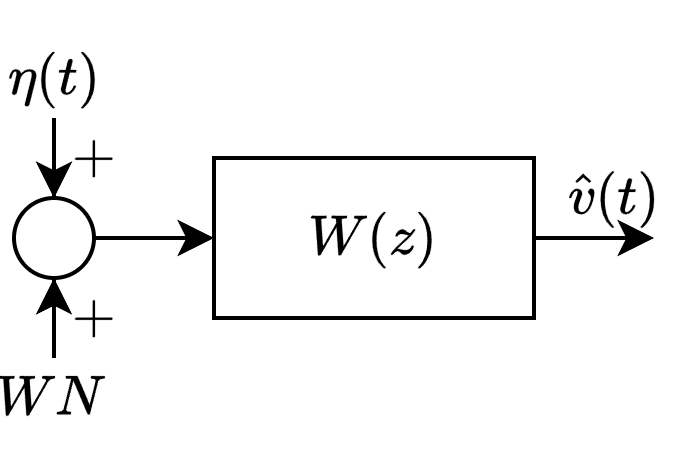
\includegraphics[width=0.3\linewidth]{images/ndet.png} 
\end{figure}
Let's visualize this with a linear time-invariant system featuring an input signal $u(\cdot)$ and an output signal $y(\cdot)$, characterized by the transfer function $W(z)$. 
According to the superposition principle, the output comprises two components: the free motion $y_{free}(\cdot)$ and the forced motion $y_{forced}(\cdot)$: 
\[y(t)=y_{free}(t)+y_{forced}(t)\]
Here, the forced motion is expressed as:
\[y_{forced}(t)=\sum_{j=t_0}^{t}w(t-j)u(j)\]
In this equation, $w(i)$ represents the impulse response samples of the system.
In the context of an asymptotically stable system, the free motion tends towards zero over time:
\[\lim_{t_0 \rightarrow -\infty}y(t)=y_{forced}(t)=\sum_{-\infty}^t w(t-j)u(j)\]
his implies that regardless of the initial conditions, as $t_0$ approaches negative infinity, the output converges to:
\[y(t)=\sum_{i=0}^{\infty}w(i)\eta(t-i)\]

\subsection{MA process}
We define the moving average process MA($n$) of order $n$ as the stochastic process represented by the equation:
\[v(t) = c_0\eta(t) + c_1\eta(t-1) + \dots + c_n\eta(t-n)\]
Here, $\eta \sim WN(0, \lambda^2)$, and  $c_0, c_1,\dots, c_n$ are real numbers.
In simpler terms, $v(t)$ is obtained by taking a weighted average of the current and past values of the white noise process $\eta$ over a time window from $t$ to $t-n$.
As time progresses, this window shifts, hence the term moving average.

For this process, the mean value is calculated as:
\begin{align*}
    \mathbb{E}\left[v(t)\right] &= \mathbb{E}\left[c_0\eta(t) + c_1\eta(t-1) + \dots + c_n\eta(t-n)\right] \\
                                &= c_0\mathbb{E}\left[\eta(t)\right] + c_1\mathbb{E}\left[\eta(t-1)\right] + \dots + c_n\mathbb{E}\left[\eta(t-n)\right] \\
                                &= 0
\end{align*}
And the variance is given by:
\begin{align*}
    \text{Var}\left[v(t)\right] &= \mathbb{E}\left[\left(v(t)-\mu(t)\right)^2\right] \\
                                &= \mathbb{E}\left[\left( c_0\eta(t) + c_1\eta(t-1) + \dots + c_n\eta(t-n) \right)^2\right] \\
                                &= \mathbb{E}\left[\left( c_0\eta(t) \right)^2 + \left(c_1\eta(t-1) \right)^2 + \dots + \left(c_n\eta(t-n) \right)^2 + \dots + \underbrace{\text{cross terms}}_0  \right] \\
                                &= c_0^2\mathbb{E}\left[\left(\eta(t)\right)^2\right] + c_1^2\mathbb{E}\left[\left(c_1\eta(t-1) \right)^2\right] + \dots + c_n^2\mathbb{E}\left[\left(c_n\eta(t-n) \right)^2\right] \\        
                                &= \left(c_0^2 + c_1^2 + \dots + c_n^2\right)\lambda^2                        
\end{align*}
Both the mean value and the variance remain constant, indicating that the process is stationary.

As for the auto-covariance, we have:
\begin{align*}
    \gamma\left[t,t+1\right]    &= \mathbb{E}\left[v(t)v(t+1)\right] \\
                                &= \mathbb{E}\left[\left( c_0\eta(t) + \dots + c_n\eta(t-n) \right)\left( c_0\eta(t+1) + \dots + c_n\eta(t-n+1) \right)\right] \\
                                &= \mathbb{E}\left[ c_0c_1 \eta(t)^2 \right] + \mathbb{E}\left[ c_1c_2 \eta(t-1)^2 \right] + \mathbb{E}\left[ c_{n-1}c_n \eta(t-n+1)^2 \right] + \dots + \underbrace{\text{cross terms}}_0   \\
                                &= c_0c_1\mathbb{E}\left[  \eta(t)^2 \right] + c_1c_2\mathbb{E}\left[  \eta(t-1)^2 \right] + c_{n-1}c_n\mathbb{E}\left[  \eta(t-n+1)^2 \right] \\        
                                &= \left(c_0c_1 + c_1c_2 + \dots + c_{n-1}c_n\right)\lambda^2                        
\end{align*}
In the general case, we find:
\[\gamma(t,t+\tau)=\mathbb{E}\left[v(t)v(t+\tau)\right]=\begin{cases}
    \left(c_0c_\tau + c_1c_{\tau+1} + \dots + c_{n-\tau}c_n\right)\lambda^2    \qquad \tau \leq n \\
    0 \qquad \tau > n
\end{cases}\]
The covariance depends solely on the difference between the two time indices.
Since the mean value and the variance are constant, and the auto-covariance depends only on the time index difference, the MA process of any finite order $n$ is weakly stationary.
Moreover, if $\eta(\cdot)$ is a Gaussian process, then $v(\cdot)$ is also a Gaussian process since it arises from a linear combination of Gaussian variables.

\paragraph*{Transfer function}
We can derive the transfer function as follows:
\begin{align*}
    v(t)    &= c_0\eta(t) + c_1\eta(t-1) + \dots + c_n\eta(t-n) \\
            &= c_0\eta(t) + c_1z^{-1}\eta(t) + \dots + c_nz^{-n}\eta(t) \\
            &= \left(c_0 + c_1z^{-1} + \dots + c_nz^{-n}\right)\eta(t) \\                  
\end{align*}
This simplifies to:
\[W(z)=c_0 + c_1z^{-1} + \dots + c_nz^{-n}=\dfrac{c_0z^n + c_1z^{n-1} + \dots + c_n}{z^n}\]
All poles of this function are at $z=0$, indicating that the system is asymptotically stable.

The MA($n$) process is characterized by $n+2$ parameters, but this representation is redundant. 
To mitigate this redundancy, parameter $c_0$ is typically set to ($C(z)$ becomes a monic polynomial).

\paragraph*{Infinite order}
When the value of $n$ tends to infinity, the expected value remains zero, but the variance:
\[\text{Var}\left[v(t)\right]=\left( \sum_{i=0}^\infty c_{i}^{2}\right) \lambda^2\]
may either converge or diverge. 
The variance is finite if and only if:
\[\sum_{i=0}^\infty c_i^2 < \infty\]
This condition not only ensures a finite variance but also guarantees that all elements of $\gamma(\tau)$ are finite, thus establishing the process as stationary.

The MA($\infty$) process possesses an auto-covariance function of infinite length, allowing it to model any stationary stochastic process. 
However, its practical utility is hindered by the challenge of handling an infinite number of parameters and the necessity for series calculations to derive $\gamma(\tau)$. 

\subsection{AR process}
The autoregressive process AR($n$) of order $n$ is represented by the equation:
\[v(t)=a_1v(t-1)+a_2v(t-2)+\dots+a_nv(t-n)+\eta(t)\]
Here, $\eta(cdot)\sim WN(0,\lambda^2)$. 

\paragraph*{Transfer function}
The transfer function can be derived as follows:
\begin{align*}
    v(t)    &= a_1v(t-1)+a_2v(t-2)+\dots+a_nv+\eta(t) \implies \\
    \eta(t) &= v(t) - a_1v(t)z^{-1} - a_2v(t)z^{-2} - \dots - a_nv(t)z^{-n} \\
            &= v(t)\left( 1 - a_1z^{-1} - a_2z^{-2} - \dots - a_nz^{-n}\right) 
\end{align*}
From this expression, the transfer function $W(z)$ is derived as:
\[W(z)=\dfrac{1}{1 - a_1z^{-1} - a_2z^{-2} - \dots - a_nz^{-n}}\]
In its standard form, $W(z)$ is represented as:
\[W(z)=\dfrac{z^n}{z^n - a_1z^{n-1} - a_2z^{n-2} - \dots - a_n}\]
Here, the denominator polynomial is denoted as $A(z)$. 

\paragraph*{Stability}
The AR(1) model is described by the equation:
\[v(t) = av(t-1) + \eta(t)\]
Consider a specific time point $t_0$ where the value of $v$ is known as $v(t_0) = v_0$.
Iterating the equation allows computing subsequent values:
\begin{itemize}
    \item $t_0 \rightarrow v(t_0) = v_0$
    \item $t_0+1 \rightarrow v(t_0+1) = av(t_0) + \eta(t_0+1) = av_0 + \eta(t_0+1)$
    \item $t_0+2 \rightarrow v(t_0+2) = av(t_0+1) + \eta(t_0+2) = a^2v_0 + a\eta(t_0+1) + \eta(t_0+2)$
\end{itemize}
In general, for $t > t_0$: 
\[v(t)=\sum_{i=t_0}^{t-1}a^{t-1-i}\eta(i+1)+a^{t-t_0}v_0\]
This system has the transfer function $A(z)=za$. 
The only root is $a$ thus the condition for asymptotic stability requires $\left\lvert a \right\rvert < 1$. 

When $t_0$ tends to $-\infty$ and the system is asymptotically stable, $v(t)$ becomes an infinite linear combination of current and past noise values, forming an MA($\infty$) process. 
The expected value is trivially null.
The variance of $v(t)$ is: 
\begin{align*}
    \text{Var}\left[v(t)\right] &= \left( (a^0)^2+(a^1)^2+(a^2)^2+\dots \right) \lambda^2 \\
                                &= \left( 1+a^2+a^4+\dots \right) \lambda^2 \\
                                &= \dfrac{1}{1-a^2} \lambda^2
\end{align*}
Since $\sum_{j=0}^{\infty}a^{2j}=\dfrac{1}{1-a^2}<\infty$, the variance is finite, and $v(t)$ indeed represents a well-defined stationary MA($\infty$) process with $c_j = a^j$. 

The auto-covariance function can be obtained using the expression for MA processes:
\[\gamma(\tau)=\lambda^2\sum_{j=0}^{\infty}c_jc_{j+\tau}=\dfrac{\lambda^2a^\tau}{1-a^2}\]

\paragraph*{AR and MA equivalence}
Since the AR(1) process is equivalent to an MA($\infty$) process, its transfer function $W(z)$ can be represented as:
\[W(z)=\dfrac{z}{z-a}=w_0+w_1z^{-1}+w_2z^{-2}+\dots\]
The coefficients $w_i$ can be computed by dividing the numerator of $W(z)$ by its denominator, yielding:
\[W(z)=\dfrac{z}{z-a}=1+\dfrac{a}{z-a}=1+az^{-1}+\dfrac{a^2z^{-1}}{z-a}=\dots\]

\paragraph*{Higher order}
The insights gained from analyzing the AR(1) process extend to autoregressive processes of arbitrary order $n$. 
An AR($n$) model that is asymptotically stable corresponds to an MA($\infty$) process, indicating stationarity.
As $t_0$ tends to $-\infty$, the solution of the time domain equation converges asymptotically to a stationary process.

Let's consider the specific case of a second-order autoregressive process:
\[v(t) = a_1v(t-1) + a_2v(t-2) + \eta(t)\]
By utilizing Yule-Walker's equations, we can determine the auto covariance function $\gamma$ of the process.  

Multiplying both sides of the equation by $v(t-\tau)$ and taking expectations leads to:
\[\gamma(\tau)=a_1\gamma(\tau-1)+a_2\gamma(\tau-2)+\mathbb{E}\left[ \eta(t)v(t-\tau) \right]\]
For the AR(2) process, this results in the following equations:
\[ \begin{cases}
    \gamma(0) = a_1\gamma(1) + a_2\gamma(2) + \lambda^2 \\
    \gamma(1) = a_1\gamma(0) + a_2\gamma(1) \\ 
    \gamma(2) = a_1\gamma(1) + a_2\gamma(0)
\end{cases} \]
Solving this system of equations allows determining $\gamma(0)$, $\gamma(1)$, $\gamma(2)$ given the parameters $a_1$, $a_2$, $\lambda^2$.
Similar equations can be derived for autoregressive processes of higher orders, such as the generic AR($n$) process.

\subsection{ARMA process}
The series combination of an autoregressive and a moving average model is described by the equation ARMA($n_a$, $n_c$), given by:
\[v(t)=a_1v(t-1) + a_2v(t-2) + \dots + a_{n_a}v(t-n_a) + c_0\eta(t) + c_1\eta(t-1) + \dots + c_{n_c}\eta(t-n_c)\]
Here, $\eta(\cdot) \sim WN(0, \lambda^2)$. 
This can be visually represented as:
\begin{figure}[H]
    \centering
    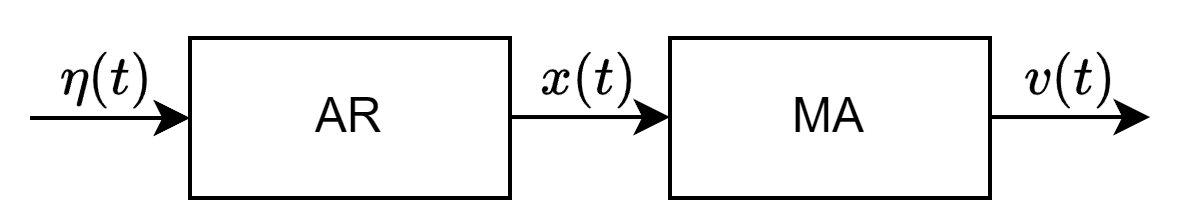
\includegraphics[width=0.5\linewidth]{images/arma.png} 
    \caption{ARMA process representation}
\end{figure}
Considering the series connection, we have:
\begin{itemize}
    \item Autoregressive process: $x(t) = a_1x(t-1) + a_2x(t-2) + \dots + a_{n_a}x(t-n_a) + \eta(t)$.
        Rewritten as a transfer function:
        \[A(z)=1-az^{-1}-\dots-a_{n_a}z^{-n_a}\]
    \item Moving average process: $v(t) = c_0x(t) + c_1x(t-1) + \dots + c_{n_c}x(t-n_c)$.
        Rewritten as a transfer function:
        \[C(z)=c_0+c_1z^{-1}+\dots+c_{n_c}z^{-n_c}\]
\end{itemize}
The transfer function of the two processes in series is given by:
\[v(t)=\dfrac{C(z)}{A(z)}\eta(t)=\dfrac{c_0+c_1z^{-1}+\dots+c_{n_c}z^{-n_c}}{1-az^{-1}-\dots-a_{n_a}z^{-n_a}}\eta(t)\]
The stability of the process depends solely on the roots of $A(z)$. 
If the transfer function is asymptotically stable, then the process generated by this equation is stationary.
\begin{example}
    Consider an ARMA(1,1) process described by the equation $v(t) = av(t-1) + \eta(t) + c\eta(t-1)$. 
    The corresponding transfer function is given by:
    \[W(z)=\dfrac{1+cz^{-1}}{1-az^{-1}}\]
    If $\left\lvert a\right\rvert  < 1$, the solution of this equation converges to a stationary process. 
    In this case, the expected value must be constant:
    \[\mathbb{E}\left[v(t-1)\right]=\mu\]
    Its value can be calculated as follows:
    \begin{align*}
        \mathbb{E}\left[v(t-1)\right] &= \mathbb{E}\left[av(t-1)+\eta(t)+c\eta(t-1)\right] \\
                                      &= a\mathbb{E}\left[v(t-1)\right]+\mathbb{E}\left[\eta(t)\right]+c\mathbb{E}\left[\eta(t-1)\right]
    \end{align*}
    Substituting, we have:
    \[\mu=a\mu+0+c\cdot 0 \rightarrow \mu=0\]
    For the variance, we compute:
    \[\text{Var}\left[v(t)\right] =\mathbb{E}\left[\left( av(t-1)+\eta(t)+c\eta(t-1) \right)^2\right]\] 
    By developing the squares we obtain:   
    \begin{multline*}
        \text{Var}\left[v(t)\right] =\mathbb{E}\left[(av(t-1))^2\right] +\mathbb{E}\left[(\eta(t))^2\right]+\mathbb{E}\left[(c\eta(t-1))^2\right] + 2a\mathbb{E}\left[ v(t-1)\eta(t) \right] \\+ 2ac \mathbb{E}\left[v(t-1)\eta(t-1)\right] + 2c\mathbb{E}\left[\eta(t)\eta(t-1)\right]
    \end{multline*}
    From which we obtain: 
    \begin{multline*}
        \text{Var}\left[v(t)\right] =a^2\underbrace{\mathbb{E}\left[v(t-1)^2\right]}_{\text{Var}\left[v(t)\right]} +\underbrace{\mathbb{E}\left[\eta(t)^2\right]}_{\lambda^2} +c^2\underbrace{\mathbb{E}\left[\eta(t-1)^2\right]}_{\lambda^2} +2a\underbrace{\mathbb{E}\left[ v(t-1)\eta(t) \right]}_{0} \\ + 2ac \underbrace{\mathbb{E}\left[v(t-1)\eta(t-1)\right]}_{\lambda^2} + 2c\underbrace{\mathbb{E}\left[\eta(t)\eta(t-1)\right]}_{0}  \\
    \end{multline*}
    Finally, we obtain: 
    \[\text{Var}\left[v(t)\right]=\dfrac{1+c^2+2ac}{1-a^2}\lambda^2\]
    Furthermore, we have:
    \[\gamma(1)=\dfrac{a + ac^2 + a^2c+c}{1-a^2}\lambda^2\]
\end{example}

\paragraph*{The vanishing covariance property}
The AR, MA, and ARMA processes share the property that as the lag $\tau$ approaches infinity, the auto covariance function $\gamma(\tau)$ tends to zero:
\[\lim_{\tau \rightarrow \infty} \gamma(\tau)=0\]
Here are the specific cases:
\begin{itemize}
    \item For MA($n$) processes, $\gamma(\tau) = 0$ for $\tau > n$.
    \item For an AR(1) process, it's known that $\gamma(\tau)=a^\tau\gamma(0)$, implying the vanishing property due to $\left\lvert a \right\rvert  < 1$.
    \item For an AR($n$) process, we can derive the Yule-Walker equation:
        \[A(z)\gamma(\tau)=0\]
        This equation suggests that $\gamma(\cdot)$ can be interpreted as the output of a system with transfer function $\frac{1}{A(z)}$ and null input.
        Under the stability condition, the output of such a system must tend to zero.
    \item For ARMA($n_a, n_c$) processes, the Yule-Walker equation remains valid for sufficiently large values of $\tau$ $(\tau > n_c)$, leading to the same consequence as the AR process.
\end{itemize}

\subsection{ARMAX process}
The models we've explored thus far are effective for describing time series data but lack the capability to represent phenomena influenced by external variables (exogenous variables).

An extension to these models is the ARMAX model, where we denote the process as $y(\cdot)$ to align with input-output system notation:
\[A(z)y(t)=B(z)u(t-k)+C(z)\eta(t)\]
Here, $u(t)$ represents the input variable, $k$ is the input-output delay, and $B(z)=b_0+b_1z^{-1}+\dots+b_{n_b}z^{n_b}$. 
\begin{figure}[H]
    \centering
    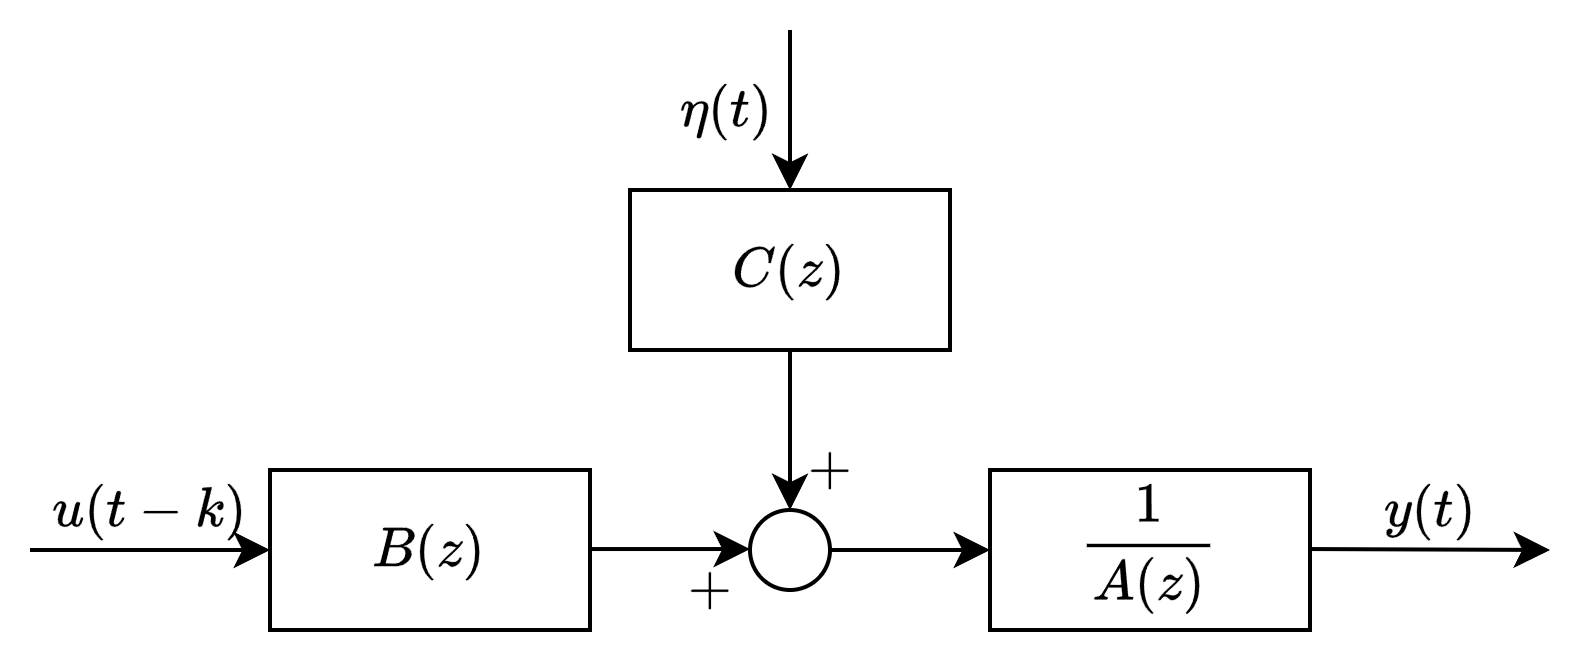
\includegraphics[width=0.5\linewidth]{images/armax.png} 
    \caption{ARMAX process representation}
\end{figure}
The core concept is to model the process through an input-output relationship while accommodating model uncertainty through the influence of white noise input.

\subsection{NARMAX process}
A further extension leads us to the nonlinear domain with the NARMAX model:
\[y(t) = f(y(t-1), \dots, y(t-n_a), u(t-k), \dots, u(t-k-n_b), \eta(t), \dots, \eta(t-n_cc))\]
Here, $f(\cdot)$ represents a nonlinear parametric function.
\begin{figure}[H]
    \centering
    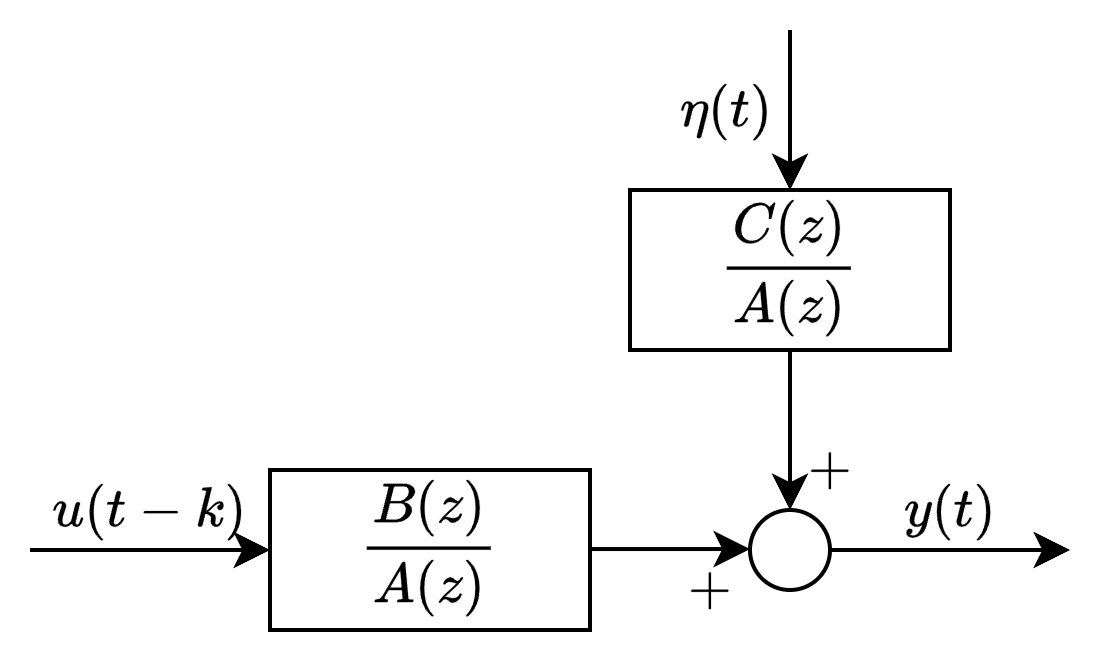
\includegraphics[width=0.4\linewidth]{images/narmax.png} 
    \caption{NARMAX process representation}
\end{figure}